%% -*- coding:utf-8 -*-
\begin{figure}
\centering

\ifpdf
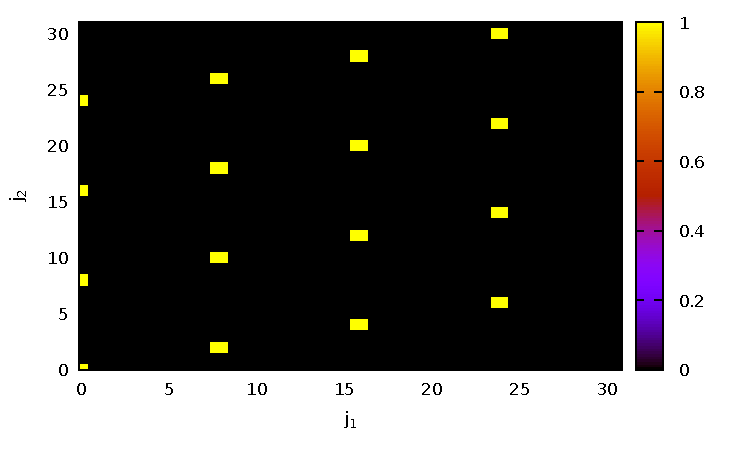
\includegraphics[angle=0]
{./part4/quantcomp/picdiscretlog2.pdf}
\else
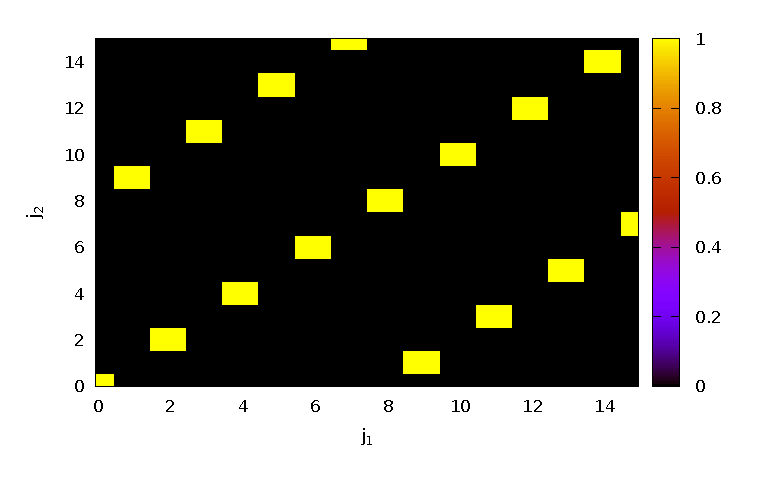
\includegraphics[angle=0]
{./part4/quantcomp/picdiscretlog2.eps}
\fi

%\input ./part4/quantcomp/picdiscretlog2.tex

\caption{Фурье образ функции с \autoref{fig:part4:quantcomp:dl1}.
  Число отсчетов $M=16$. Координаты максимума $j_1 = 9$, $j_2 = 1$. 
Решением уравнения $3^x \equiv 14 \mod 17$
является $x = \frac{9}{1} = 9$} 
\label{fig:part4:quantcomp:dl2}
\end{figure}
